
\chapter{Hemholtz散射系数介绍}
\label{chapter:ref1}
在本章,我们将对声波Hemholtz散射系数加以介绍,其目的是为了说明在第二章所提半空间无相位数据成像算法\ref{alg_phaseless},对于嵌入在半空间中的不可穿透障碍物,仅仅能够对其上半边界进行有效成像。除此之外,散射系数的引入同样解释如下现象:第三、四章针对Pekeris开波导模型所提的算法\ref{alg_wg}和算法\ref{alg_imp},在对嵌入在Pekeris开波导第二层的不可障碍物进行成像时,同样仅仅能够确定障碍物的上半边界。

关于散射系数或反射系数的研究文献有很多,例如Richard B.Melrose\cite{Melrose1985Near},David Colton\cite{colton-kress},以及Habib Ammari\cite{Ammari2013Enhancement,Ammari2013The,Ammari2015Super,Hirst2013Enhancement}。特别地,我们参考文献\cite[Definition 4.1]{ch_ha}的定义,具体如下:
\begin{definition}\label{scatter_coeff}
假设声软障碍物$D\subset\R^2$为有界Lipschitz区域,然后令$\eta\in S^1$为单位向量,其表示入射场$e^{\i kx\cdot\eta}$的入射方向,并设$v^s(x,\eta)$为如下方程的散射解:
\begin{eqnarray}
\left\{
\begin{array}{lll}
\Delta v^s(x,\eta)+k^2v^s(x,\eta)=0,&in&\R^2\backslash\overline{D},\\
& &\\
v^s(x,\eta)=-v^i(x,\eta),& on& \Gamma_D,\\
& &\\
\sqrt{r}\left(\frac{\partial v^s}{\partial r}-\i kv^s\right)\rightarrow0,& as& r\rightarrow\infty,\ \ r=|x|.
\end{array}
\right.
\end{eqnarray}
其中常数$k$为背景波数,则散射系数$R(x,\eta),x\in\Gamma_D,\eta\in S^1$,由如下关系所定义:
\begin{equation}
\frac{\partial(v^s+v^i)}{\partial\nu}=\i kR(x,\eta)e^{\i kx\cdot\eta},\ \ on\  \ \Gamma_D.
\end{equation}
\end{definition}
\begin{remark}
根据文献\cite{colton-kress,cc14}中关于全空间Hemholtz散射问题的适定性研究可知,定义\ref{scatter_coeff}中关于散射系数$R(x,\eta)$的引出是合理而明确的。
\end{remark}
文献\cite{ch_ha}指出,当$D$是严格凸的障碍物时,根据Kirchhoff高频渐进假设,例如文献\cite{bcs,Melrose1985Near},可知散射系数$R(x,\eta)$可以被下式所近似:
\begin{eqnarray}\label{kir_app}
  R(x,\eta)=
  \left\{
\begin{array}{lll}
2\nu(x)\cdot\eta,&if&x\in\partial D^-_{\eta}:=\{x\in\Gamma_D:\nu(x)\cdot\eta<0\},\\
0,&if&x\in\partial D^+_{\eta}:=\{x\in\Gamma_D:\nu(x)\cdot\eta>0\}
\end{array}
  \right.
\end{eqnarray}
其中$\partial D^-_{\eta}$和$\partial D^+_{\eta}$分别表示照明区域和阴影区域。

下面我们对定义\ref{scatter_coeff}和高频近似\ref{kir_app}做一下对比,不妨设$D$是一个圆形障碍物,其边界$\Gamma_D$参数表达为:$x_1=\rho\cos\theta,x_2=\rho\sin\theta,\theta\in(0,2\pi)$,那么在点$x\in\Gamma_D$的法向为$\nu(x)=(\cos\theta,\sin\theta)$。记入射方向$\eta=(\cos\beta,\sin\beta),\beta\in(0,2\pi)$,则散射系数$R(x,\eta)$可记为
\begin{equation}
 \hat R(\theta,\beta):=R(x(\theta),\eta(\beta)),\  \ \theta,\beta\in(0,2\pi)
\end{equation}

图\ref{com_kir_def1}和图\ref{com_kir_def2}表明了:当频率$k$比较大时,Kirchhoff高频近似\ref{kir_app}确实为定义\ref{scatter_coeff}中散射系数$R(x,\eta)$的一个很好的近似。

\begin{figure}[htbp]
	\centering
	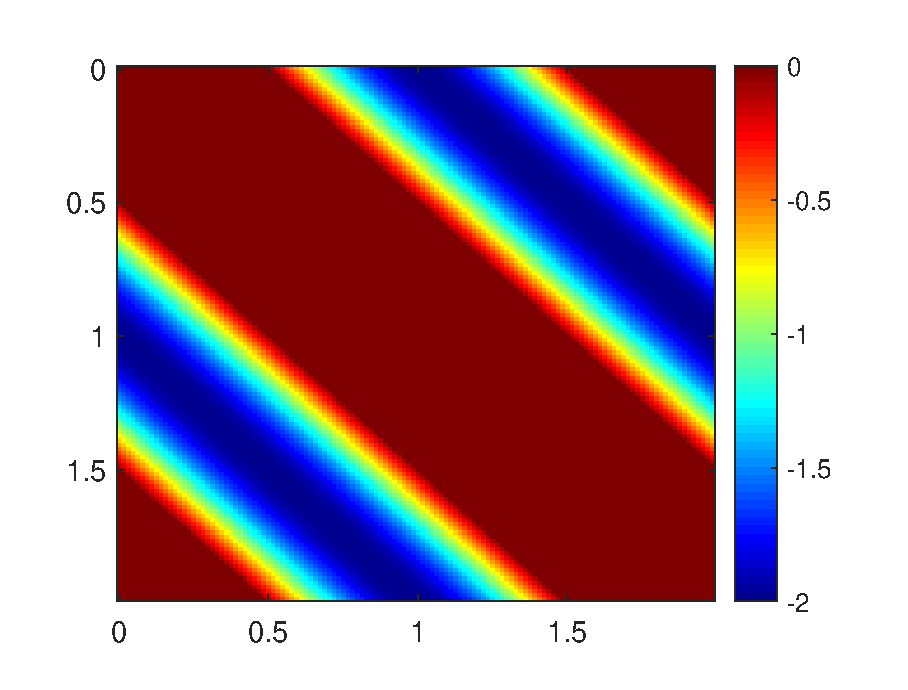
\includegraphics[width=0.4\textwidth]{./scatter_coeff/kirchhoff}
	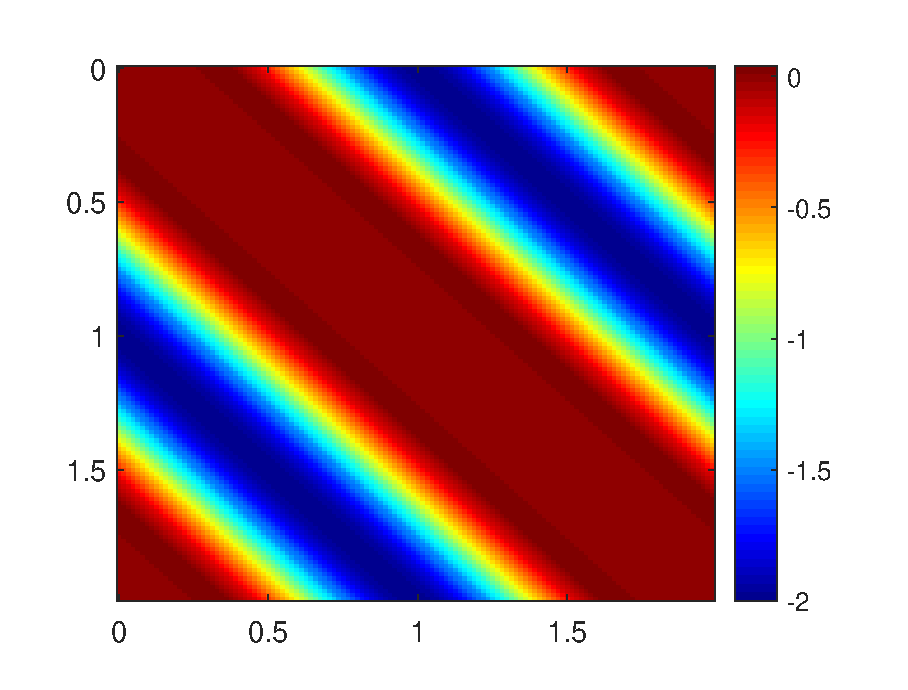
\includegraphics[width=0.4\textwidth]{./scatter_coeff/definition}
	\caption{高频情形散射系数定义与Kirchhoff逼近对比示意图:左边对应于定义\ref{scatter_coeff},右边对应于Kirchhoff高频近似\ref{kir_app}。其中横坐标表示$\frac{\theta}{2\pi}$,纵坐标表示$\frac{\beta}{2\pi}$,颜色深浅表示$\hat R(\theta,\beta)$的具体数值。具体参数:波数$k=8\pi$,$D$的半径$\rho=1$。}\label{com_kir_def1}
\end{figure}
\begin{figure}[htbp]
	\centering
	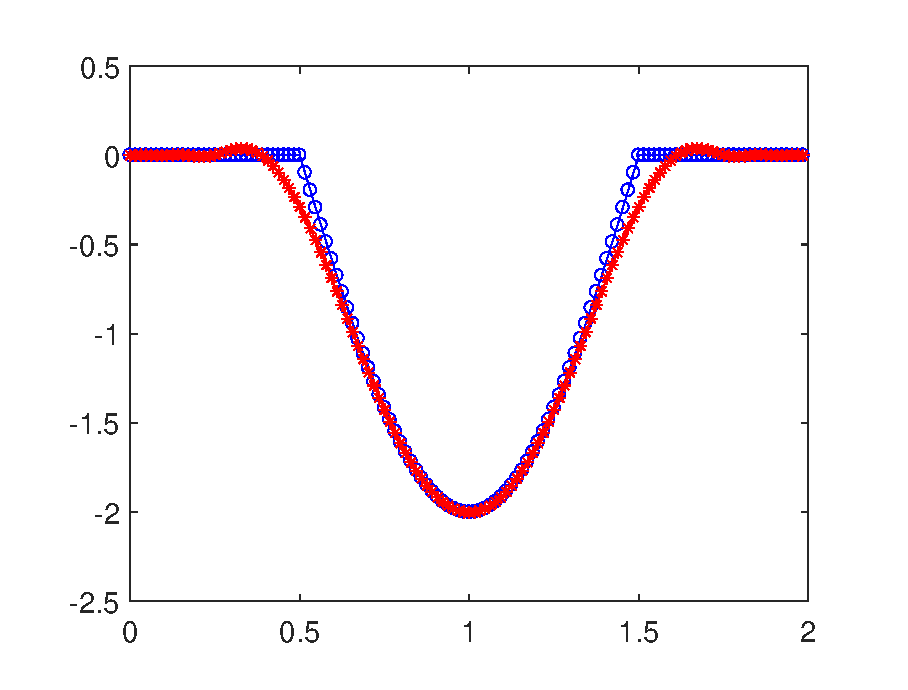
\includegraphics[width=0.4\textwidth]{./scatter_coeff/eta0}
	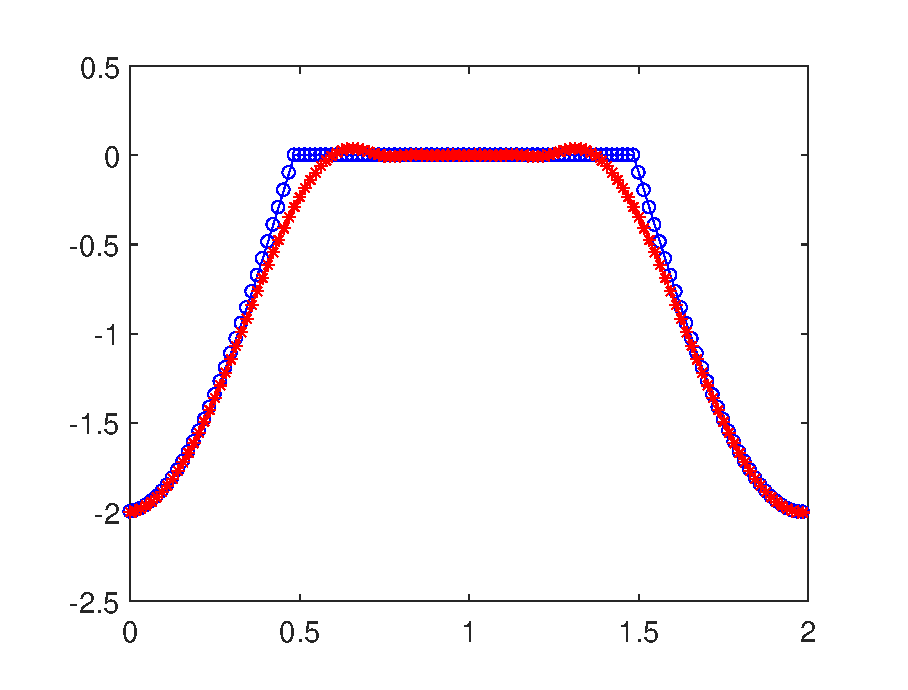
\includegraphics[width=0.4\textwidth]{./scatter_coeff/etapi}
	\caption{高频情形散射系数定义与Kirchhoff逼近对比示意图:左边表示入射角度为$\theta=0$时, $\hat R(\theta,\eta)$随$\eta\in(0,2\pi)$的变化情况。其中横坐标表示$\frac{\eta}{2\pi}$,纵坐标表示$\hat R(\theta,\beta)$的具体数值;红色为通过定义\ref{scatter_coeff}所计算出的散射系数,蓝色为Kirchhoff高频近似\ref{kir_app}。右边为入射角度$\theta=\pi$时相应的结果。具体参数:波数$k=8\pi$,$D$的半径$\rho=1$。}\label{com_kir_def2}
\end{figure}

散射系数的分析和测试表明:在相对于入射场$v^i(x,\eta):=e^{\i kx\cdot\eta}$的阴影区域,即$\nu(x)\cdot\eta>0$时,散射系数几乎为零。这就解释了本章开始所提到的针对不可穿透障碍物数值测试所遇到的现象:如果仅仅在半空间边界$\Gamma_0$上放置激发点源以及接受数据,那么数值重构算法仅能够确定不可穿透障碍物的上边界。